\chapter{The Software Build Process}
%Die Aufgabe des Erstellungs- (od. Build)-Prozesses in der
%SW-Entwicklung ist es, die
%benötigten Produkte (Artefakte) in einer konsistenten,
%reproduzierbaren und soweit wie möglich
%automatisierten Weise zu erstellen.

Build is the process of creating the application program for a
software release, by taking all the relevant source code files
and compiling them and then creating a build artefact, such as
binaries or executable program, etc.\\

The build process should be automated as much as possible and
be reproducible.\\

You can also say that the build process is a combination of
several activities which varies for each programming language
and for each operating system but please remember the basic
concepts are universal.\\

\vspace{3mm}

The build process could include the following activities:

%In der Regel umfasst
%dieser Prozess die folgenden Schritte:

\begin{itemize}
\item Fetching the code from source control repository
\item Compile the code and check dependencies
\item Run automated unit tests
\item Link the libraries, code etc accordingly
\item Build artifacts
\item Deploy application
\item Generate documentation
\item Archive build logs
\end{itemize}

To have the possibility to create an automated and reproducible
process, a description of each software (e.g. compiler) including
parameters and dependencies is needed.\\

\vspace{3mm}

The build process is \structure{CRISP} oriented.

%Der Erstellungsprozess soll sich am Prinzip \structure{CRISP} orientieren:

 {\bfseries C}omplete {\bfseries R}epeatable {\bfseries I}nformative {\bfseries S}chedulable {\bfseries P}ortable

Typical tools which could be used are::
\begin{itemize}
\item make, CMake and Automake/Autotools (Unix, Windows/Cygwin)
\item Apache Ant
\item Apache Maven
\item Gradle
\end{itemize}
%
\section{Apache Ant}
Apache Ant is a Java library and command-line tool whose mission
is to drive processes described in build files as targets and
extension points dependent upon each other. The main known usage
of Ant is the build of Java applications. Ant supplies a number of
built-in tasks allowing to compile, assemble, test and run Java
applications. Ant can also be used effectively to build non Java
applications, for instance C or C++ applications. More generally,
Ant can be used to pilot any type of process which can be described
in terms of targets and tasks.\\

\vspace{3mm}

To use Apache Ant, a build file in XML format is needed. This file
has the following prooperties:

%Um Ant zu verwenden, muss eine sogenannte Build-Datei in XML-Format erstellt
%werden. Diese Datei hat folgende Eigenschaften:
\begin{itemize}
\item Each build file contains one project
\item Each project contains one or more {\bfseries Targets}. Each Target
will execute a given number of {\bfseries Tasks}.
\end{itemize}
\newslide
Sample build file:
\begin{lstlisting}[language=xml,morekeywords={project,target,javac,mkdir}]
<project name="SimpleProject" default="compile">

  <target name="init">
    <mkdir dir="build"/>
  </target>

  <target name="compile" depends="init">
    <javac srcdir="src"
        destdir="build"/>
  </target>
</project>
\end{lstlisting}
\ifslides
\else
This build files takes care that
%Die obige Datei sorgt dafür, dass
\begin{enumerate}
\item the directory \verb|build| will be created (if not already there).
\item all Java source code files which are in the \verb|src| directory
  will be compiled and the result will be written to the \verb|build| directory.
\end{enumerate}
\fi
\newslide
%Ein Ant-Prozess kann wie folgt angestossen werden:
A process based on Ant could be started in the following way:

\begin{tabularx}{\linewidth}{l|X}
Call   & Description \\
\hline
ant  &  will execute the default target in the build file (build.xml)\\
%\hline
ant -f otherbuild.xml & using a different name for the build file: otherbuild.xml\\
%\hline
ant compile & executes the target {\bfseries compile}
  aus.\\
%\hline
ant -projecthelp & displays all available targets\\
%\hline
ant -version & displays the current Ant version\\
%\hline
ant -emacs & creates Emacs based log statements.\\
\end{tabularx}

Per default, Ant contains about 80 tasks. Most of the work which
needs to be done in the build process could be covered with the
default tasks. Default tasks are:
\begin{itemize}
\item Copy
\item Create directory
\item Create jar file
\item Compile code
\item Execute operating system command
\end{itemize}
There is also the possibility to extend Ant with your own tasks.
Many extension projects are available.

%Standardmässig bringt Ant über 80 Tasks mit, die einen breiten
%Anwendungsbereich abdecken und die auch durch eigene Tasks erweitert werden
%können. Es gibt über 100 Erweiterungsprojekte und Tools zu Ant.
%
\newslide
\subsection{Constants}
Whenever possible, make use of properties in your build file:
%Um allenfalls notwendige Anpassungen zu vereinfachen, sollten in der
%Build-Datei Konstanten als sogenannte Properties vereinbart werden:
\begin{lstlisting}[language=xml, morekeywords={property,target,javac}]
<property name="build.dir" value="build"/>
<target name="compile">
  <javac srcdir="src"
        destdir="${build.dir}"/>
</target>
\end{lstlisting}
%$
Properties could be defined in an additional file or in the build file
directly:
%Oft sind diese auch in einer separaten Datei definiert:
\begin{lstlisting}[language=xml,morekeywords={property}]
<property file="project.properties"/>
\end{lstlisting}
The project.properties file contains key value pairs:
%In der Datei project.properties sind die Werte zeilenweise aufgeführt:
\begin{verbatim}
build.dir=build
\end{verbatim}
%
\newslide
\subsection{Create Jar file}
A jar file could be created with the jar task:
%Eine Archiv-Datei kann mit dem Task jar erstellt werden:
\begin{lstlisting}[language=xml,morekeywords={target,jar,mkdir}]
<target name="dist" depends="compile"
   description="generate the distribution" >
   <mkdir dir="dist" />
   <jar destfile="dist/project.jar"
        basedir="${build.dir}"/>
</target>
\end{lstlisting}
%$
The attribute destfile defines the final file name and the
basedir defines, which files should be included.


%Das Attribut destfile legt den Filenamen fest und mit basedir wird
%das Verzeichnis bezeichnet, dessen Dateien in die Archiv-Datei
%aufgenommen werden.

\newslide
To create an executable jar file, the following manifest needs to be
added:
%Um eine Archiv-Datei ausführbar zu machen, muss eine Manifest-Datei
%mit folgendem Inhalt hinzugefügt werden:
\begin{verbatim}
  Main-Class: classname
\end{verbatim}
classname is the class, which contains the \verb|main| method. There
is a possibility to do that directly in the Ant task:
%wobei \verb+classname+ die Klasse bezeichnet, welche die Main-Methode
%enthält. In der Ant-Build-Datei kann dies mit dem Element manifest
%vereinbart werden:
\begin{lstlisting}[language=xml,morekeywords={jar,manifest,attribute}]
   <jar destfile="dist/project.jar"
        basedir="${build.dir}">
      <manifest>
	<attribute name="Main-Class"
		   value="example.Main"/>
      </manifest>
   </jar>
\end{lstlisting}
%$
\newslide
\subsection{Fileset}
Filesets are used as a common way to bundle files:
%Mit Filesets können Dateien gruppiert werden:
\begin{lstlisting}[language=xml,morekeywords={fileset,include,exclude}]
<fileset dir="src">
  <include name="**/*.java"/>
  <exclude name="**/*Test*"/>
</fileset>
\end{lstlisting}
A group will be created, containing all files from the \verb|src| directory ending with \verb|.java|
or containing the word \verb|Test| in the filename.
%Hiermit wird eine Gruppe gebildet mit allen Java-Dateien, die im
%src-Verzeichnis und darunter liegen und nicht den Text ''Test'' im
%Namen enthalten.
%
\newslide
\subsection{Path}
A path is a collection of resources (files). A path has an id and could
then be used within another task:
%Als Pfad bezeichnet man eine Sammlung von Ressourcen (Dateien), die
%üblicherweise mit einem Id-Attribut eindeutig gekennzeichnet werden:
\begin{lstlisting}[language=xml,morekeywords={path,pathelement,fileset,include}]
<path id="compile.classpath">
  <fileset dir="lib">
    <include name="**/*.jar"/>
  </fileset>
</path>

<path id="run.classpath">
  <pathelement location="${build.dir}"/>
  <path refid="compile.classpath"/>
</path>
\end{lstlisting}
%$
\newslide
This approach is used to set the classpath in the compilation process:
%Damit kann beim Compilieren der Klassenpfad wie folgt gesetzt werden:
\begin{lstlisting}[language=xml,morekeywords={javac,classpath}]
<javac ...>
  <classpath refid="compile.classpath"/>
</javac>
\end{lstlisting}
%
\newslide
\subsection{Exercise}
\begin{enumerate}
\item Create an Ant build file for the loader project. This build file
should contain the following targets:
\begin{itemize}
\item clean (delete all generated artifacts)
\item compile (compiles the java code)
\item dist (creates an executable jar file, containing the build date)
\end{itemize}

\end{enumerate}
%
\newslide
\subsection{Software and further Informations}
\begin{itemize}
\item Java Development with Ant (Erik Hatcher, Steve Loughan), Manning
  Publications
\item Das Apache ANT Projekt:
  \href{http://ant.apache.org}{ant.apache.org}
\item Apache Ant:
  \href{http://en.wikibooks.org/wiki/Programming:Apache_Ant}
     {en.wikibooks.org/wiki/Programming:Apache\_Ant}
\item Ant Wiki:
  \href{http://wiki.apache.org/ant/FrontPage}{wiki.apache.org/ant/FrontPage}
\item Introduction to
  Ant:\href{http://www.exubero.com/ant/antintro-s5.html}
{www.exubero.com/ant/antintro-s5.html}
\end{itemize}
%
\newslide
%
% http://pettermahlen.com/2010/05/01/code-sharing-use-maven/
%

\newpage

\section{Maven}
Wie Ant ist auch Maven ein Open-Source-Werkzeug zur einfachen Automatisierung von
Build-Prozessen.

\ifslides
Vorteile:
\begin{itemize}
\item Reduzierter Konfigurationsaufwand:
       {\em deklarativ} statt {\em imperativ}, Convention over Configuration
\item Paket-Management mit Versionierung: Repository für Libraries
\item Einheitlicher Build-Prozess mit Standardverzeichnisstruktur
\item IDE-Unabhängigkeit: Unterstützung von Eclipse, Netbeans, Intellij
\end{itemize}
\else
Im Unterschied zu Ant basiert Maven jedoch auf einem
{\em deklarativen} anstelle eines {\em imperativen} Ansatzes:
man beschreibt {\em was} und
nicht {\em wie} man etwas tun will. Die Folge davon ist ein
wesentlich geringerer Konfigurationsaufwand.
Zusätzlich orientiert sich Maven am Prinzip ``Convention over
Configuration'': hält man sich an die von Maven vorgeschlagene
Verzeichnisstruktur, vereinfacht sich die Konfiguration entsprechend.

Eine weitere wertvolle Eigenschaft von Maven ist die Fähigkeit
die verwendeten Bibliotheken (sog. Artefakte) zu verwalten.
Maven holt sich bei Bedarf
die benötigten Archivdateien vom Internet herunter und legt sie
in ein zentrales Repository.

Von Haus aus bringt Maven bereits
einen Standard-Build-Prozess mit und etabliert damit
eine einheitliche Projektstruktur. Auch dies ein nicht zu
unterschätzender Vorteil. Ausserdem kann Maven unabhängig von einer IDE
benutzt werden, es unterstützt aber auch die
Entwicklungsumgebungen Eclipse, Netbeans und Idea.

Die erste Version von Maven, die 2002 in relativ kurzer Zeit
eingeführt wurde, wies noch einige Unzulänglichkeiten
auf. Mittlerweile ist eine in wesentlichen Teilen erneuerte und
verbesserte Version 2 (resp. 3) verfügbar. Diese Versionsproblematik
kann jedoch auf einigen Internet-Seiten noch für etwas Verwirrung
sorgen.
\fi
\newslide
%
\subsection{Projektmodell}
Grundlage des Erstellungsprozesses von Maven ist das Projektmodell (POM).
Es beschreibt die Metadaten, Abhängigkeiten und alle notwendigen
Angaben damit Maven den entsprechenden Build-Prozess
durchführen kann:
\begin{itemize}
\item \structure{Allgemeine Angaben}: Projektkoordinaten, Verpackungsart \ldots
\item \structure{Dependencies}: Abhängigkeiten zu externen Bibliotheken,
\item Build: spezielle Angaben zum Build-Prozess (plugins),
\item Properties: projekt-spezifische Konstanten,
\item Profile: Build-Varianten,
\item Repositories: spezielle Verzeichnisse für die verwendeten
  Bibliotheken und Plugins,
\item Reporting: Projektdokumentation
\end{itemize}
Diese Angaben werden in der XML-Datei pom.xml abgelegt. Beispiel:
\begin{lstlisting}[language=xml,
   morekeywords={modelVersion,groupId,artifactId,
   packaging,version,name,url,dependencies,dependency,scope,project}]
  <project xmlns="http://maven.apache.org/POM/4.0.0"
       xmlns:xsi="http://www.w3.org/2001/XMLSchema-instance"
       xsi:schemaLocation="http://maven.apache.org/POM/4.0.0
                  http://maven.apache.org/maven-v4_0_0.xsd">
  <modelVersion>4.0.0</modelVersion>

  <groupId>example</groupId>
  <artifactId>myapp</artifactId>
  <packaging>jar</packaging>
  <version>1.0-SNAPSHOT</version>

  <name>My First App</name>
  <url>http://maven.apache.org</url>

  <dependencies>
    <dependency>
      <groupId>junit</groupId>
      <artifactId>junit</artifactId>
      <version>3.8.1</version>
      <scope>test</scope>
    </dependency>
  </dependencies>
</project>
\end{lstlisting}
\newslide
Die allgemeinen Angaben werden mit den folgenden Elementen beschrieben:
\begin{itemize}
\item \structure{groupId}: der eindeutige Bezeichner der Projektorganisation
  (meist ein DNS-Bezeichner, z.B. org.apache.maven)
\item \structure{artifactId}: der eindeutige Bezeichner des erzeugten
  Ergebnisses, z.B: myapp
\item \structure{version}: die Version des Artefaktes
\item \structure{packaging}: die Verpackungsart des Artefaktes
\item \structure{name}: der in der Dokumentation verwendete Projektbezeichner
\item \structure{url}: die Web-Seite des Projektes
\end{itemize}
Unter dependencies findet man
das junit-Artefakt, welches im Projekt für die Test-Phase
benötigt wird. Hier können weitere Dependency-Elemente
hinzugefügt mit Scope den jeweiligen Verwendungsbereich
 (test, compile, provided, runtime, system) vereinbart werden.
%
% Lat. ars „Bearbeitung“ und factum „das Gemachte“
% Artefakt:
% in der Softwareentwicklung ein Produkt, das als Zwischen- oder
% Endergebnis der Softwareentwicklung entsteht
%
\newslide
% http://www.avajava.com/tutorials/lessons/what-are-the-phases-of-the-maven-default-lifecycle.html
\subsection{Build-Lifecycle}
Leicht vereinfacht ist der Build-Prozess bei Maven
in die folgenden Phasen gegliedert:
\begin{itemize}
\item \structure{process-resources}: Konvertierung der Ressource-Dateien,
%(korrekte, vollständige Projektstruktur),
\item \structure{compile}: Kompilation des Quellkodes,
\item \structure{test}: Durchführung von Tests,
\item \structure{package}: Verpackung der Dateien,
\item \structure{integration-test}: Installation in eine Testumgebung zur
  Durchführung der Integrationstests,
\newslide
%\item \structure{verify}: Überprüfung der Gültigkeit,
\item \structure{install}: Installation in das lokale Maven-Repository,
\item \structure{deploy}: Installation in die Integrations-
                        oder Release-Umgebung,
 kopiert das Paket in das  Remote-Repository, so dass es von anderen
 Projekten verwendet werden kann,
\end{itemize}
%Diese Phasen werden in der dargestellten Reihenfolge durchgeführt. Das
%heisst, wenn man zum Beispiel \verb+package+ ausführen lassen möchte,
%werden zuerst die davor liegenden Phasen validate, compile, und test
%ausgeführt.
%
Darüberhinaus stellt Maven die folgenden Funktionen bereit:
\begin{itemize}
\item \structure{clean}: löscht alle generierten Dateien,
\item \structure{site}: erzeugt die Projekt-Dokumentation
\end{itemize}
\newslide
Abhängig vom jeweiligen Projekttyp
 sind jeder Projektphase eine Anzahl
von Aktionen (sogenannte Goals),
die als Maven-Plugins implementiert sind, zugeordnet.

Typischerweise wird der Projekttyp durch die Verpackungsart
festgelegt: jar, war, ear oder pom sind gültige Beispiele.

\newslide
Mit der JAR-Verpackung sind
folgende 8 Phasen mit ihren Plugins und Goals verknüpft:

\begin{tabularx}{\linewidth}{llll}
  & Phase &  Plugin & Goal\\
\hline
1 & process-resources & maven-resources-plugin & resources:resources\\
2 & compile & maven-compiler-plugin & compiler:compile\\
3 & process-test-resources & maven-resource-plugin & resources:testResources\\
4 & test-compile & maven-compiler-plugin & compiler:testCompile\\
5 & test & maven-surefire-plugin  & surefire:test\\
6 & package & maven-jar-plugin & jar:jar\\
7 & install & maven-install-plugin & install:install\\
8 & deploy & maven-deploy-plugin & deploy:deploy\\
\end{tabularx}
%
\newslide
\subsection{Vorgehen}
Das grundsätzliche Vorgehen mit Maven wird im Folgenden anhand eines einfachen
Java-Projektes (sog. Artefakt), welches die Bibliotheken junit und
log4j verwendet, erläutert:
\begin{enumerate}
\item \underline{Erstellung der Projektstruktur:}
  \begin{lstlisting}
% mkdir projects
% cd projects
% mvn archetype:generate -Dfilter=quickstart
  \end{lstlisting}
  Die Ausführung kann beim ersten Mal etwas Zeit beanspruchen,
  da dabei einige Dateien in das lokale
  Repository \verb+~/.m2/repository+ kopiert werden.

  Mit dem Argument \verb+archetype:generate+ wird der Aktionsblock
  \verb+generate+ des Maven-Plugins \verb+archetype+ ausgeführt.
  Aktionsblöcke werden als Goals bezeichnet.

  Jedes Artefakt ist durch seine Koordinaten eindeutig identifiziert:
  \begin{itemize}
  \item \structure{groupId}: Paketbezeichner (Namespace), Name der Organisation
  \item \structure{artifactId}: Projektbezeichner
  \item \structure{version}: Versionsbezeichner,
    Defaultwert ist: \verb+1.0-SNAPSHOT+, welcher den
  Entwicklungsstatus bezeichnet (d.h. das Ergebnis wird kontinuierlich
  aktualisiert).
  \begin{figure}[H]
  \begin{center}
  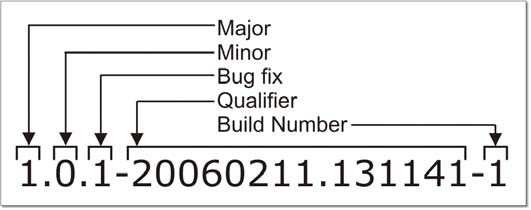
\includegraphics[width=0.65\linewidth]{config-management/major-minor}
  \end{center}
  \caption{Format des Versionsbezeichners (Source: Better Builds mit Maven)}
  \end{figure}
\newslide
Beispiele gültiger Versionsbezeichner:
  \begin{itemize}
  \item 1.0.1-20080211.131141-1
  \item 1.0-alpha
  \item 1.0
  \end{itemize}
  \end{itemize}
  Einige Artefakt-Beispiele:
\begin{center}
\begin{tabular}{lll}
groupId & artifactId & version\\
\hline
junit  & junit & 3.8.1\\
log4j & log4j & 1.2.13\\
mysql & mysql-connector-java & 5.1.5\\
org.springframework & spring & 2.5\\
\end{tabular}
\end{center}
Weitere (aktuell gibt es einige 1000 groupIds) findet man im
offiziellen Maven-Repository:
\href{http://mirrors.ibiblio.org/maven2}{mirrors.ibiblio.org/maven2}

\newslide
Hiermit ist nun die in Abbildung \ref{fig:maven-dirstruct} gezeigte
Verzeichnisstruktur entstanden.
\begin{figure}[H]
  \centering
\ifslides
  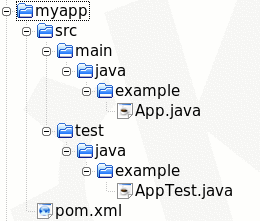
\includegraphics[width=0.4\linewidth]{config-management/maven-dirstruct}
\else
  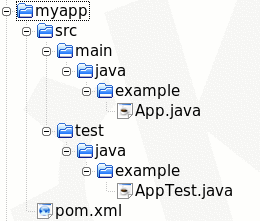
\includegraphics[width=0.4\linewidth]{config-management/maven-dirstruct}
\fi
  \caption{Verzeichnisstruktur eines Maven-Projektes}
  \label{fig:maven-dirstruct}
\end{figure}
\newslide
Mit archetype:generate wird eine Auswahl möglicher Projektvorlagen präsentiert, die mit dem Argument -Dfilter
eingegrenzt werden kann.
%
\newslide
\item \underline{Compilieren und Testen}

Man kann nun auf der Kommandozeile die Aktionen einer bestimmten Projektphase
ausführen. Zum Beispiel:
\begin{lstlisting}
  % mvn test
\end{lstlisting}
Hiermit werden ohne weiteres Zutun die Aktionen aller Phasen bis und
mit der Test-Phase durchgeführt, d.h. es werden die benötigten
Bibliotheken, sofern
nicht vorhanden, heruntergeladen,
die Dateien kompiliert und anschliessend die Unit-Tests
durchgeführt. Dazu werden die Standard-Plugins von Maven verwendet, die
beispielsweise bei Java-Code den Java-1.5-Compiler verwenden.
\newslide
Will man jedoch
 spezifische Compiler-Flags benutzen, muss dies dem
 Plugin \verb+maven-compiler-plugin+ mitgeteilt werden:
\begin{lstlisting}[language=xml,
  morekeywords={plugins,plugin,configuration,artifactId,source,target}]
  <plugins>
    <plugin>
      <artifactId>maven-compiler-plugin</artifactId>
      <configuration>
        <source>1.8</source>
        <target>1.8</target>
      </configuration>
    </plugin>
  </plugins>
\end{lstlisting}
Das Plugins-Element ist Teil des Build-Elementes.
\newslide
\item \underline{Weitere Artefakte verwenden:}

Benötigt man weitere Bibliotheken, dann müssen diese der Dependency-Liste
  hinzugefügt werden. Beispiel:
  \begin{lstlisting}[language=xml,
    morekeywords={dependency,groupId,artifactId,version,scope}]
 <dependency>
   <groupId>log4j</groupId>
   <artifactId>log4j</artifactId>
   <version>1.2.13</version>
   <scope>compile</scope>
 </dependency>
  \end{lstlisting}
Das Maven-Repository kann mit
\href{https://search.maven.org}{search.maven.org}
%\href{http://maven.ozacc.com}{http://maven.ozacc.com} oder
%\href{http://mvnbrowser.com}{mvnbrowser.com}
durchsucht werden.

Maven sorgt dann dafür, dass die entsprechenden Dateien in das lokale
Repository kopiert werden.
%
\newslide
\item \underline{Ausführen}

Das Ausführen gehört nicht eigentlich zu den Kern-Kompetenzen von
Maven. Mit dem Exec-Plugin kann jedoch eine Java-Applikation  wie
folgt ausgeführt werden:
\begin{lstlisting}
mvn exec:java -Dexec.mainClass=example.App
\end{lstlisting}
Allfällige Argumente können mit \verb+-Dexec.args=".."+ übergeben
werden.

Das Exec-Plugin kann auch konfiguriert werden:
\begin{lstlisting}[language=xml,
  morekeywords={plugin,groupId,artifactId,configuration,mainClass}]
<plugin>
  <groupId>org.codehaus.mojo</groupId>
  <artifactId>exec-maven-plugin</artifactId>
  <configuration>
    <mainClass>example.App</mainClass>
  </configuration>
</plugin>
\end{lstlisting}
\newslide
\item \underline{Verpacken:}

Mit dem Parameter package erstellt Maven entsprechend der
Packaging-Property eine Java-Archiv-Datei, die im Verzeichnis
target abgelegt wird. Dabei werden allerdings die abhängigen
Archiv-Dateien nicht mit verpackt. Dies wird vielmehr vom Assembly-Plugin
übernommen:
\begin{lstlisting}[language=xml,
  morekeywords={plugin,artifactId,configuration,descriptorRefs,
  descriptorRef}]
  <plugin>
    <artifactId>maven-assembly-plugin</artifactId>
    <version>3.1.0</version>
    <configuration>
      <descriptorRefs>
        <descriptorRef>jar-with-dependencies</descriptorRef>
      </descriptorRefs>
    </configuration>
  </plugin>
\end{lstlisting}
\newslide
Dieses Plugin ermöglicht es zudem, das Main-Class-Attribut
des Manifests zu definieren:
\begin{lstlisting}[language=xml,
morekeywords={configuration,archive,manifest,mainClass}]
..
    <configuration>
      ..
      <archive>
        <manifest>
          <mainClass>myapp.Main</mainClass>
        </manifest>
      </archive>
      ..
    </configuration>
 ..
\end{lstlisting}
% mvn npackage assembly:single
Die Aktion (das Goal) {\bfseries assembly:single} sorgt
für die eigentliche Erstellung der Archiv-Datei.
Um diese Aktion
 mit der Package-Phase zu verknüpfen, muss das
Execution-Element wie folgt konfiguriert werden:
\begin{lstlisting}[language=xml,
  morekeywords={executions,execution,id,phase,goals,goal}]
  <executions>
    <execution>
      <id>make-assembly</id>
      <phase>package</phase>
      <goals>
        <goal>single</goal>
      </goals>
    </execution>
  </executions>
\end{lstlisting}
Hiermit wird beim Aufruf von Maven mit dem Parameter {\bfseries package} die
Jar-Datei, welche alle Klassen der zu diesem Artefakt abhängigen
Archiv-Dateien enthält.
%
\newslide
\item \underline{Installieren:}

Maven installiert die erstellten Erzeugnisse (Artefakte) in das lokale (private)
Repository und macht sie damit für eigene Maven-Projekte verfügbar:
\begin{lstlisting}
  mvn install
\end{lstlisting}
Bei einer Jar-Datei wird der Pfadname folgt gebildet:
\begin{verbatim}
<groupId>/<artifactId>/<version>/<artifactId>-<version>.jar
\end{verbatim}
Beispiel: org/example/myapp/1.0-SNAPSHOT/myapp-1.0.SNAPSHOT.jar
%
\newslide
\item \underline{Deployment:}

Beim Deployment werden die Artefakte in ein entferntes Repository
kopiert. Dazu werden verschiedene Verfahren unterstützt: File-Copy,
FTP und SCP/SSH.
Zur Konfiguration dient das DistributionManagement-Element:
\begin{lstlisting}[language=xml,
  morekeywords={distributionManagement,repository,id,name,url}]
  <distributionManagement>
    <repository>
      <id>internal.repository</id>
      <name>Internal Repository</name>
      <url>file://${basedir}/target/deploy</url>
    </repository>
  </distributionManagement>
\end{lstlisting}
Bei FTP und SCP/SSH müssen Benutzername/Passwort resp. Public-Key in
der benutzer-spezifischen Settings-Datei \verb+~/.m2/settings.xml+
definiert werden.
\end{enumerate}
% $
\newslide
\subsection{Verwendung von Property-Werten}
Properties werden wie bei Ant für
Werte verwendet, die an verschiedenen Stellen referenziert werden:
\begin{lstlisting}[language=xml,
 morekeywords={dependencies,dependency,groupId,artifactId,
   version,scope,properties,junit}]
  <dependencies>
    <dependency>
      ...
      <version>${junit.version}</version>
    </dependency>
  </dependencies>

<properties>
  <junit.version>3.8.1</junit.version>
</properties>
\end{lstlisting}
% $
\newslide
Maven kennt eine Vielzahl implizit definierter Properties:

\begin{tabularx}{\linewidth}{lX}
\verb+project.*+ & Elemente des POM: project.name, project.version\\
\verb+settings.*+ & Benutzerabhängige Maven-Setting-Elemente\\
\verb+env.*+ & Umgebungsvariablen: env.M2\_HOME, env.PATH \\
System Properties & Java-System-Properties: os.name, java.home \ldots\\
\end{tabularx}
\newslide
\subsection{Erstellungsvarianten mit Build-Profiles}
Mit Hilfe des Profile-Elementes können unterschiedliche
Erstellungsvarianten konfiguriert werden:
\begin{lstlisting}[language=xml,
  morekeywords={profiles,profile,id,build,plugins,plugin,artifactId,
    configuration,debug,optimize}]
  <profiles>
    <profile>
      <id>production</id>
      <build>
	<plugins>
          <plugin>
            <artifactId>maven-compiler-plugin</artifactId>
	    <configuration>
	      <debug>false</debug>
	      <optimize>true</optimize>
	    </configuration>
	  </plugin>
	</plugins>
      </build>
    </profile>
  </profiles>
\end{lstlisting}
Ein bestimmtes Profile kann mit Angabe des Id-Bezeichners bei der
Ausführung mit der Option -P von Maven festgelegt werden:
\begin{lstlisting}
  mvn -Pproduction compile
\end{lstlisting}
\newslide
\subsection{Filtern von Ressourcen}
Für die einfache Anpassung umgebungsabhängiger Konstanten und Texte werden
bei Java-Programmen in der Regel spezielle Ressourcen-Dateien verwendet.
Zum Beispiel können damit der Name und die Version einer Applikation
gesetzt werden:
\begin{lstlisting}[language=java]
  ResourceBundle rb =
     ResourceBundle.getBundle("ApplicationResources");

  String appname = rb.getString("application.name");
  String version = rb.getString("application.version");
  System.out.println("This is " + appname +
                     " (Version " + version + ")");
\end{lstlisting}
\newslide
Legt man im Verzeichnis src/main/resources die Datei
ApplicationResources.properties mit folgendem Inhalt ab
\begin{lstlisting}
# application resources
application.name=${project.name}
application.version=${project.version}
\end{lstlisting}
dann kann Maven dafür sorgen, dass die Property-Werte in der
process-resources-Phase aus der POM-Datei übernommen und eingesetzt
werden.
\newslide
Dazu muss jedoch das
Resource-Element entsprechend konfiguriert werden:
\begin{lstlisting}[language=xml,
morekeywords={build,resources,resource,directory,filtering}]
   <build>
     <resources>
       <resource>
	 <directory>src/main/resources</directory>
	 <filtering>true</filtering>
       </resource>
     </resources>
  </build>
\end{lstlisting}
\newslide
%Die Variable Project enthält die POM-Werte
%
\subsection{Test-Durchführung}
Die Durchführung der Unit-Tests ist Bestandteil des
Standard-Build-Prozesses, für welches das Plugin
maven-surefire-plugin zuständig ist:
\begin{lstlisting}
mvn test
\end{lstlisting}
Ohne entsprechende Konfiguration werden alle Tests in den Dateien des
Verzeichnisses src/test und aller Unterverzeichnisse mit folgendem
Muster ausgeführt:
\begin{itemize}
\item \verb+**/Test*.java+
\item \verb+**/*Test.java+
\item \verb+**/*TestCase.java+
\end{itemize}
Dabei können die Testklassen mit TestNG, Junit oder sogar
als normale POJO-Klassen
implementiert werden. Das Plugin berücksichtigt dazu die entsprechende
Dependency-Konfiguration.

Die Ergebnisse werden als
Report-Dateien jeweils in Text- und XML-Format ins Verzeichnis
target/surefire-reports abgelegt und der Build-Prozess wird
abgebrochen, falls ein Unit-Test fehlschlägt.

Dieses Verhalten kann jedoch konfiguriert werden:
\begin{lstlisting}[language=xml,
  morekeywords={plugin,groupId,artifactId,configuration,testFailureIgnore,includes}]
  <plugin>
    <artifactId>maven-surefire-plugin</artifactId>
    <configuration>
      <includes>**/*</includes>
      <testFailureIgnore>false</testFailureIgnore>
    </configuration>
  </plugin>
\end{lstlisting}
%
\newslide
\subsection{Reporting}
Mit der Anweisung:
\begin{lstlisting}
% mvn site
\end{lstlisting}
erzeugt Maven eine Projekt-Dokumentation, die im Verzeichnis target/site
abgelegt wird. Die dazu nötigen Informationen werden ebenfalls der
POM-Datei entnommen. Zum Beispiel:
\begin{lstlisting}[language=xml,morekeywords={name,url,description}]
..
  <name>My first Project powered by maven</name>
   <url>http://your.project.url</url>
   <description>Write some brief explanatory text
             about your project.</description>
..
\end{lstlisting}
Das Layout der so erzeugten Dokumentation
kann mit dem File src/site/site.xml angepasst werden.

\newslide
\begin{figure}[H]
\centering
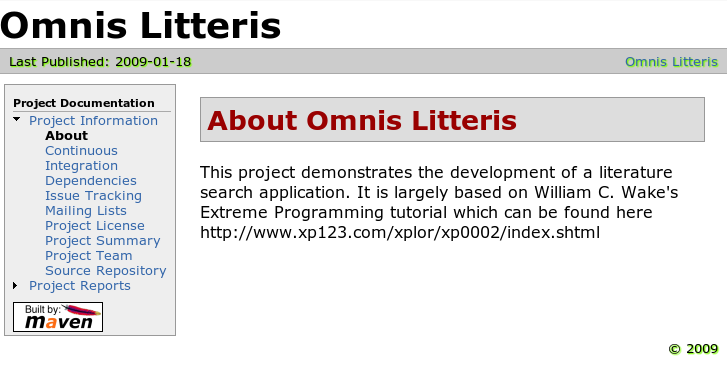
\includegraphics[width=\linewidth]{config-management/mvnsite}
\caption{Eine mit Maven erstellte Projektseite}
\end{figure}
\newslide
Für eine umfassende Dokumentation sorgen zahlreiche Plugins (Beispiele):
\begin{itemize}
\item Change-Log: maven-changelog-plugin
\item Checkstyle: maven-checkstyle-plugin
\item Junit-Report: maven-surefire-report-plugin
\item PMD: maven-pmd-plugin
\item Findbugs: findbugs-maven-plugin
\item JavaDoc: maven-javadoc-plugin
\item Cobertura: cobertura-maven-plugin
\item JXR (Cross-Reference): maven-jxr-plugin
\end{itemize}
\newslide
\begin{lstlisting}[language=xml,
  morekeywords={reporting,plugins,plugin,groupId,artifactId,
    version,configuration}]
  <reporting>
    <plugins>
      <plugin>
	<groupId>org.codehaus.mojo</groupId>
	<artifactId>cobertura-maven-plugin</artifactId>
      </plugin>
      <plugin>
	<artifactId>maven-javadoc-plugin</artifactId>
      </plugin>
      <plugin>
	<artifactId>maven-jxr-plugin</artifactId>
      </plugin>
 ..
    </plugins>
  </reporting>
\end{lstlisting}
\newslide
%\newpage
\newslide
\subsection{Eigene Dateien hinzufügen}
Das (lokale) Maven-Repository kann auch mit eigenen Dateien oder solchen,
die man von dritter Seite erhalten hat, ergänzt werden:
\begin{lstlisting}
mvn install:install-file     \
     -Dfile=Sample.jar       \
     -DgroupId=uniquesample  \
     -DartifactId=sample_jar \
     -Dversion=2.1.3b2       \
     -Dpackaging=jar         \
     -DgeneratePom=true
\end{lstlisting}
%
\newslide
\subsection{Software Version Control (SCM)}
Mit Hilfe des Plugins \verb+maven-scm-plugin+
bietet Maven auch eine einheitliche Schnittstelle zu
den Source-Code-Management (SCM) Systemen CVS, SVN, GIT (u.a.) an:
\begin{center}
\begin{tabular}{l|l}
Aktion & Beschreibung\\
\hline
 scm:checkin & Änderungen zum SCM-Repository senden\\
 scm:checkout & Arbeitskopie erstellen\\
 scm:add     & Datei hinzufügen\\
 scm:update  & Dateien aktualisieren \\
 scm:status & Status anzeigen\\
 scm:tag    & eine Markierung setzen\\
 \ldots
\end{tabular}
\end{center}
Bei einigen Aktionen müssen Parameter angegeben werden:
\begin{lstlisting}
  % mvn -Dmessage="<checkin comment here>" scm:checkin
\end{lstlisting}
Dazu muss in der POM-Datei das Element scm definiert werden:
\begin{lstlisting}[language=xml,
  morekeywords={scm,connection,developerConnection,url}]
<scm>
  <developerConnection>
    scm:svn:https://somerepository.com/svn_repo/trunk
  </developerConnection>
</scm>
\end{lstlisting}
Bei GIT lautet die URL wie folgt (Beispiel):
\begin{lstlisting}
  scm:git:git://github.com/path_to_repository
\end{lstlisting}
Weitere Infos: \href{http://maven.apache.org/scm/git.html}
                    {maven.apache.org/scm/git.html}
\newslide
\subsection{Release-Bildung}
Bei der Release-Bildung überprüft das Release-Plugin die folgenden Punkte:
\begin{itemize}
\item Sind alle lokalen Änderungen mit dem SCM-Repository abgeglichen?
\item Sind alle Integrations-Tests fehlerfrei durchgelaufen?
\item Werden bei den verwendeten Bibliotheken und Plugins
  keine SNAPSHOT-Versionen referenziert?
\end{itemize}
und sorgt dafür, dass die Versionsbezeichner in den POM-Dateien
entsprechend angepasst werden und mit den SCM-Tags korrespondieren:
\begin{lstlisting}
mvn release:prepare -DdryRun=true
\end{lstlisting}
\newslide
Das Plugin verlangt anschliessend die folgenden Angaben:
\begin{itemize}
\item aktueller Versionsbezeichner (Bsp: 1.0)
\item aktueller Releasebezeichner (Bsp: myapp-1.0)
\item neuer Bezeichner der Entwicklungsversion (Bsp: 1.1-SNAPSHOT)
\end{itemize}
und legt die eingebenen Werte in der Datei release.properties
ab. Zusätzlich werden verschiedene POM-Dateien erzeugt, die man
allesamt mit
\begin{lstlisting}
mvn release:clean
\end{lstlisting}
wieder löschen muss, wenn Maven die Aktionen ausführen soll.
\newslide
Nach Eingabe von
\begin{lstlisting}
mvn release:prepare
\end{lstlisting}
% achtung: bei SVN 1.5.2:
%    svn: Commit failed (details follow):
%    svn: File '..' already exists
%
% svn update und ein erneutes mvn:prepare behebt das Problem
%
wird Maven den aktuellen Stand des Projektes in das Tags-Verzeichnis
kopieren, die neue Versionsbezeichnung
in den POM-Dateien einsetzen und mitteilen, dass man nun mit
\begin{lstlisting}
mvn release:perform
\end{lstlisting}
die eigentlichen Release-Dateien bilden und in das lokale (und
Deploy-) Repository
transferieren kann. Damit dieser Schritt klappt, muss das
distributionManagement-Element definiert sein.
% Achtung:
% maven-release-plugin
% configuration tag
%  <plugin>
%        <artifactId>maven-release-plugin</artifactId>
%        <configuration>
%          <tagBase>http://localhost/omnislitteris/tags
%          </tagBase>
%        </configuration>
%      </plugin>
%

Eine verbesserte Unterstützung bietet das Plugin jgitflow:
\begin{lstlisting}[language=xml,morekeywords={plugin,groupId,artifactId,configuration,noDeploy}]
<plugin>
   <groupId>external.atlassian.jgitflow</groupId>
   <artifactId>jgitflow-maven-plugin</artifactId>
   <version>1.0-m5.1</version>
   <configuration>
     <noDeploy>true</noDeploy>
   <configuration>
</plugin>
\end{lstlisting}
Plugin goals:
\begin{itemize}
\item \structure{jgitflow:release-start} create and push a release branch
\item \structure{jgitflow:release-finish} build, tag and merge the release branch
into master and develop branches
\end{itemize}
\newslide
\subsection{Exercise}
\begin{enumerate}
\item Konvertieren Sie das Projekt Histogram in ein Maven-Projekt
(artifactId: histogram, groupId=demo) und
erstellen Sie die ausführbare Archiv-Datei mit allen benötigten Klassen.
Wie lautet der Dateiname der Archiv-Datei, und wie kann man ihn
konfigurieren?

%Hinweis: Bis und mit Version 1.0.12
%wird von jfreechart  die Library gnujaxp benötigt, welche
%nicht im offiziellen Maven-Repository abgelegt ist. Sie müssen
%in diesem Fall Ihre
%POM-Datei mit dem folgenden Repositories-Element ergänzen:
%\begin{lstlisting}[language=xml,
%   morekeywords={repositories,repository,id,name,url}]
%  <repositories>
%    <repository>
%      <id>maven-repository.atlassian.com</id>
%      <name>Atlassian Maven Repository</name>
%      <url>http://maven.atlassian.com/repository/public</url>
%    </repository>
%  </repositories>
%\end{lstlisting}
\end{enumerate}
%
\subsection{Software and further Informations}
\begin{itemize}
\item Maven: \href{http://maven.apache.org/}{maven.apache.org/}
\item Maven, The Definitive Guide
%(Tim O'Brien, John Casey, Brian Fox, Bruce Snyder, Jason Van Zyl)

\href{http://www.sonatype.com/book/reference/public-book.html}
{www.sonatype.com/book/reference/public-book.html}

\item Eclipse und Maven:
  \href{http://www.eclipse.org/m2e/}{www.eclipse.org/m2e/}
%\item An introduction to Maven 2
%
%\href{http://www.javaworld.com/javaworld/jw-12-2005/jw-1205-maven.html}
%   {www.javaworld.com/javaworld/jw-12-2005/jw-1205-maven.html}
%
%\item Building Web Applications with Maven
%
%   \href{http://today.java.net/pub/a/today/2007/03/01/building-web-applications-with-maven-2.html}
%      {today.java.net/pub/a/today/2007/03/01/building-web-applications-with-maven-2.html}
%
%\item Maven 2.0: Compile, Test, Run, Deploy, and More
%
%\href{http://www.onjava.com/pub/a/onjava/2006/03/29/maven-2-0.html}
%{www.onjava.com/pub/a/onjava/2006/03/29/maven-2-0.html}
%
%\item Get the most out of Maven 2 site generation:
%
%\href{http://www.javaworld.com/javaworld/jw-02-2006/jw-0227-maven.html}
%  {www.javaworld.com/javaworld/jw-02-2006/jw-0227-maven.html}
%
%\item Introduction to Apache Maven 2
%
%\href{http://www-128.ibm.com/developerworks/edu/j-dw-java-mavenv2.html}
%   {www-128.ibm.com/developerworks/edu/j-dw-java-mavenv2.html}
%
%\item Tutorial:Hibernate, Spring, HSQL, Eclipse \& Maven
%
%\href{http://www.lulu.com/content/1087191}{www.lulu.com/content/1087191}
%
%\item Netbeans Wiki: Maven best practices
%
%\href{http://wiki.netbeans.org/MavenBestPractices}
%  {wiki.netbeans.org/MavenBestPractices}
%
%\item Working with Maven in Netbeans
%
%\href{http://today.java.net/article/2009/10/14/working-maven-netbeans-671}
%  {today.java.net/article/2009/10/14/working-maven-netbeans-671}
\end{itemize}

\newpage
